

\section*{Exercises}

\begin{exercise}
For the following functions, find $f(3)$:

\begin{itemize}
\item $f(t) = 4t$
\item $f(t) = -\frac{1}{2}t + 1$
\item $f(x) = x^2 - 2x + 1$
\item $f(x) = 2$
\item $f(z) = 7$
\item $f(z) = z^3-z^2-z-1$
\end{itemize}

\end{exercise}
\bigskip

\begin{exercise}
Build a table for the following functions:

\begin{itemize}
\item $f(t) = t + t + t + t + t$
\item $f(x) = 1-x^{2}$
\item $f(q) = q^{120}\times 0$
\end{itemize}

\end{exercise}
\bigskip

\begin{exercise}
If $f(x) = x^2$, find $x$ where $f(x) = 4$.
\end{exercise}
\bigskip

\begin{exercise}

	$f(x) = 3x + 20$
	
	Find:
	\begin{itemize}
		\item $f(-5)$
		\item $f(0)$
		\item $f(1)$
		\item $f(9001)$
	\end{itemize}
	
			Find $x$ such that:
	\begin{itemize}
		\item $f(x)=-5$
		\item $f(x)=0$
		\item $f(x)=1$
		\item $f(x)=9001$
	\end{itemize}
\end{exercise}
\bigskip

\begin{exercise}
Make a table with a column for each of the following functions, making sure to include some negative values:

\begin{itemize}
\item $f(x) = x$
\item $g(x) = x^2$
\item $h(x) = x^3$
\item $i(x) = x^4$
\end{itemize}

Describe the difference between the functions based on this table.

\end{exercise}
\bigskip

\begin{exercise}

Let 
\begin{itemize}
\item $f(x) = \frac{2}{5}x$
\item $g(x) = 2 - 3x$
\end{itemize}

Find $f(10)$, and then put that value into $g(x)$.  Then, find $g(10)$, and put that value into $f(x)$.  Compare these values.

\end{exercise}

\begin{exercise}
	Create two tables with different scales for the function $f(x) = x^2 - 9$.
\end{exercise}
\bigskip

\begin{exercise}
The following is a table of two functions

\begin{tabular}{|c|c|c|}
\hline
$x$ & $f(x)$ & $g(x)$ \\
\hline
-2 & -50 & 1\\
\hline
-1 & -2 & 3\\
\hline
0 & 14 & 10\\
\hline
1 & 16 & 3\\
\hline
2 & 15 & 1\\
\hline
\end{tabular}

What is $g(x)$ when $f(x) = -2$?

For which values of $x$ is $f(x) > g(x)$?

\end{exercise}
\bigskip

\begin{exercise}

Toaster function:

In the domain of the toaster function, we have bread, pop-tarts, and bagels, as we expect.  We also could put toast back into the toaster function, as well as the resulting charcoal.  The table would look like the following:

\begin{tabular}{|c|c|}
\hline
$x$ & toaster$(x)$\\
\hline
bread & toast\\
\hline
pop-tart & pop-tart\\
\hline
toast & charcoal\\
\hline
charcoal & ashes\\
\hline
bagel & bagel\\
\hline
\end{tabular}

What is $a$ if toaster$(a) = $ charcoal?

What is $a$ if toaster$($charcoal$)$ $ = a$?

Explain.

\end{exercise}
\bigskip

\begin{exercise}
Give three functions for which $f(5) = 0$
\end{exercise}
\bigskip

\begin{exercise}
Some sort of respiratory illness has infected some of a farmer's cattle.  He has decided to use amoxicillin to treat them.  The dosage guidelines of amoxicillin are 2 milliliters for every 100 pounds the animal weighs.  Create a table and a graph which show the relationship between the weight of an infected cow and the amount of antibiotic needed to treat it.
\end{exercise}
\bigskip

\begin{exercise}
While the sun never sets on the British empire, its control has changed appreciably over the years.  The following is a chart of the land area of the British Empire for various years.  

\begin{center}
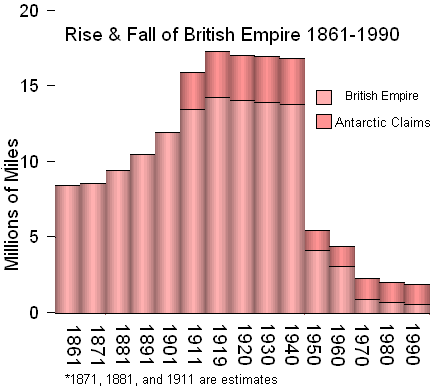
\includegraphics{images/riseandfall.png}
\end{center}

(Wikipedia: Territorial evolution of the British Empire) [1]

In what time interval is the territory of the British Empire growing?  In what time interval is it shrinking?  Let $f(t)$ be the function of land area of the British Empire over time, where $t$ is the current year.  Estimate $f(1940)$ and $f(1950)$.  Find $t$ where $f(t)$ is the highest.

\end{exercise}
\bigskip

\begin{exercise}
Liam weighs 205 pounds and is looking to put on another 10 pounds in muscle over the next 6 months.  He lifts three days per week, and his trends in the past have been to stay at the same weight with a 30-minute workout.  His gain after 6 months is usually one pound for each additional 5 minutes he works out for each session.

How long should he plan to lift each session to meet his goal?
If he plans to lift for 60 minutes each session, how much should he expect to gain in 6 months?
\end{exercise}
\bigskip

\begin{exercise}
Before the beginning of each school year, you, a teacher, need to order enough books for your students, plus a few backup copies.  There are 4 books they each need, and you want 5 replacements for each book, regardless of how many students you have.  Give an equation, table, and graph for this relationship.
\end{exercise}
\bigskip

\begin{exercise}
To set up your account with the electric company, you must pay a \$90 activation fee.  Your plan is 10 cents per kilowatt-hour.  Additionally, based on information from previous accounts, they have determined that your average bill over the year is \$70.  How much money will you give the electric company this year?  Create a table for the amount you've given the electric company as a function of time.
\end{exercise}

\begin{exercise}
You're considering subscribing to Netflix.  You don't watch very many TV shows, but you watch movies occasionally.  The main competitor for your purposes is Redbox, which rents individual movies for \$1 each.  Netflix is for \$10 each month.

Make a table of the per-month price for each Netflix and Redbox, based on the number of movies you watch each month.  How could this table influence your decision?

\end{exercise}

\begin{exercise}
A local community can estimate their corn yield per acre by keeping track of the greatest number of consecutive days without rain.  They estimate 180 bushels as a high mark, but subtract the greatest number of consecutive days without rain.

How many consecutive days without rain would the community have to have before they estimate only 140 bushels per acre?
\end{exercise}
\bigskip

\begin{exercise}
	The $3^{\prime\prime}$ cactus in my window grows at a rate of $\frac{1}{4}^{\prime\prime}$ per month.  Give an equation, table, and graph which express its height over time.
\end{exercise}
\bigskip

\begin{exercise}

The amount of gas required to start a certain engine is 8 milliliters.  This engine also consumes 0.4 milliliters of gas every second it spends idling.  Create an equation, table, and graph to express this relationship.

\end{exercise}
\bigskip

\begin{exercise}
If a baseball (or, really, any other object) is thrown upward at 40 meters per second, the following equation describes its height as a function of time:

$$f(t) = 2 + 40t - \frac{1}{2}9.8t^2$$

Create a table and a graph for the function.  Make sure to include values of $t$ from 0 to 10.  Using as few math terms as possible, describe what this function is telling us.

\end{exercise}
\bigskip


\begin{verbatim}
[1] https://en.wikipedia.org/wiki/Territorial_evolution_of_the_British_Empire#/media/File:Riseandfall1.PNG
\end{verbatim}